\chapter{Background and Related Work}
The aim of drug discovery is to find new chemical entities with desirable pharmacological properties. This is an inherently difficult task due to the vast size and complexity of the chemical search space. The range of drug-like molecules has been estimated to be between 10\textsuperscript{23} and 10\textsuperscript{60} \cite{polishchuk2013estimation}. Meanwhile, the chemical space is discrete, making the search difficult to perform \cite{kirkpatrick2004chemical}. As a result, drug development is a lengthy and costly process, with the average clinical development time for one drug reaching more than nine years and the estimated median development cost 1.1 billion USD \cite{wouters2020estimated}.

\section{Background}
Generative models, which are a type of machine learning model used to generate new data samples that are similar to a training data set, have been widely used in natural language processing (NLP) tasks \cite{shorten2021text}. Inspired by this success, researchers in the field of chemistry have applied these models to the task of generating novel chemical compounds, or molecules, with specific properties. A representation system known as the simplified molecular-input line-entry system (SMILES) has been developed to represent molecules as strings of characters \cite{meyers2021novo},\cite{weininger1988smiles}. Using this system, generative chemists used long short-term memory (LSTM) networks and recurrent neural networks (RNNs) to generate molecules via a text-based approach \cite{gupta2018generative}. In recent years, researchers have developed SMILES-based autoencoders (AEs) and variational autoencoders (VAEs) to generate molecules.

 However, the use of SMILES as a representation for molecules has some limitations. For example, different start positions and paths through the molecule can produce different SMILES, resulting in a lack of uniqueness in the description of the molecule\cite{meyers2021novo, sousa2021generative, lee2022mgcvae, li2018multi}. Additionally, text-based generative models that use SMILES must learn rules unrelated to molecular structure, such as SMILES grammar and atomic order, which can be burdensome for the training process. As a result, researchers have developed alternative representations for molecules, such as canonical SMILES, DeepSMILES, and SELFIES \cite{o2012towards,o2018deepsmiles, krenn2020self}.

To address the limitations of SMILES, researchers have suggested using graph-based representations for molecules, where atoms and bonds are represented as nodes and edges, respectively \cite{meyers2021novo, sousa2021generative, li2018multi}. Graph-based models can overcome the artificial aspects of SMILES syntax and make it easier to express essential chemical properties such as molecule validity. One example of a graph-based model is the junction tree variational autoencoder (JTVAE), which has been used to generate molecules with specific properties \cite{jin2018junction}.

\section{Related Work}
Prior work on molecular graph generation can be classified into atom-based and fragment-based models \cite{meyers2021novo}. In atom-based models, SMILES are generated before translating them into graphs via deterministic mappings using RDKIT \cite{landrum2013rdkit}. Notable atom-based models include GraphVAE and MolGAN, which learn to generate graph adjacency in a one-shot fashion. GraphVAE uses graph convolutional layers in the encoder and decoder \cite{simonovsky2018graphvae}. MolGAN combines GAN and reinforcement learning (RL) to generate outputs probabilities over the adjacency matrix and the annotation matrix of a molecular graph \cite{de2018molgan}. However, these models suffer from scalability issues, which restrict \textit{de novo} drug design to molecules with small sizes \cite{li2018multi}.

While atom-based generative models cover a wider chemical space, fragment-based approaches constrain the search space using a coarser molecular representation \cite{meyers2021novo}. The JTVAE is a pioneering approach to fragment-based models\cite{jin2018junction}. Firstly, a tree-structured scaffold of molecular substructures is generated by the VAE. Subsequently, the fragments are assembled to construct the final molecular graph. In doing so, the JTVAE could maintain chemical validity in each step. 

\section{Models}
\subsection{Variational autoencoders}
This paper focuses on graph generation autoencoder (AE) methods. Specifically, VAEs have shown great success across a broad range of applications in generative modeling and unsupervised learning tasks. A VAE is a neural network that can learn to generate new data samples that are similar to a training data set by learning a compact, low-dimensional representation of the data, called the latent space \cite{doersch2016tutorial, pu2016variational}. The VAE is derived from a standard encoder-decoder pair framework that observes a space $x$ in terms of a prior distribution over a latent space $p(z)$ and a conditional likelihood of generating a data sample from a latent space $p_\theta(x|z)$. The probabilistic encoder of a VAE maps the input to the posterior density $q_\phi(z|x)$ over the latent variable, $z$, with a multivariate Gaussian, $q_\phi(z|x)\sim\mathcal{N}(\mu_\phi,\sigma^2_\phi)$. The decoder then reconstructs the input data from the latent variable, which is given by the density $p_\theta(x|z)$. 

The VAE aims to learn the marginal log-likelihood of the observed data in the generative process. Since the log-likelihood is intractable, the evidence lower bound (ELBO) relies on the posterior distribution $q_\phi(z|x)$ to maximize the log-likelihood defined below:
\begin{equation}
\max_{\phi, \theta} \mathbb{E}_{q_\phi(z|x)}[log p_\theta(x|z)]\label{eq}
\end{equation}
where $\mathbb{E}$ is the expectation value \cite{richards2022conditional}. Equation 1 is also known as the ELBO formulation. In (1), the VAE aims to minimize the reconstruction term for the encoder to generate meaningful latent vectors which the decoder can subsequently reconstruct. The optimization objective of the VAE can be written as follows:
\begin{equation}
\mathcal{L}(\theta,\phi;x,z) = log p_\theta(x|z) - D_{KL}[q_\phi(z|x)\parallel p(z)]\label{eq}
\end{equation}
where $D_{KL}(\parallel)$ stands for non-negative Kullback-Leibler divergence loss between the true and approximate posterior. Since VAEs are gradient-based optimization approaches, it is necessary to define a differentiable loss function to update the network weights through backpropagation. In short, the VAE aims to optimize the model parameters $\theta$ to reduce the reconstruction error between the input and the output, and $\phi$ to make $q_\phi(z|x)$ as close as possible to $p_\theta(z|x)$. Since maximizing the ELBO is equivalent to maximizing the log-likelihood of the observed data and minimizing the divergence of the approximate posterior from the exact posterior, (1) and (2) can be rewritten as follows:
\begin{equation}
\begin{split}
log p_\theta(x|z) \geq & \mathcal{L}(\theta,\phi;x,z) \\= \mathbb{E}_{q_\phi(z|x)}[log p_\theta(x|z)]
& - D_{KL}[q_\phi(z|x)\parallel p(z)]. \label{eq}
\end{split}
\end{equation}
However, a standard VAE often experiences posterior collapse, in which the network learns a trivial local optimum of the ELBO objective \cite{richards2022conditional}. This means that the variational posterior is misrepresented as the true posterior. Researchers from \cite{higgins2016beta} have shown that posterior collapse could occur due to an insufficient representation of the reconstruction loss. During training, VAEs give equal weight to the reconstruction and KL loss terms, causing the network to prematurely optimize the KL factor. As a result, an inaccurate local optimum poorly approximates the true posterior.

\subsection{$\beta$-VAE}
To overcome posterior collapse, \cite{higgins2016beta} introduced the $\beta$-VAE, where the hyperparameter $\beta$ is applied during training. The $\beta$-VAE uses the principles of VAE and disentangled representation learning to generate new molecules similar to the training data set. Disentanglement refers to the separation of the latent variables in the VAE's latent space into independent dimensions that correspond to specific aspects of the data \cite{mathieu2019disentangling}. In short, multiplying the KL loss in (3) by $\beta$ penalizes the VAE for learning latent space dimensions that are highly correlated with each other \cite{burgess2018understanding}.

Tuning the $\beta$ factor controls the strength of the constraint on the latent space to be disentangled. A higher value of beta encourages the latent space to be more disentangled, while a lower value allows for more flexibility in the representation. Equation 4 shows the resulting ELBO formulation for the objective function of the $\beta$-VAE:
\begin{equation}
\begin{split}
log p_\theta(x|z) \geq & \mathcal{L}(\theta,\phi;x,z) \\= \mathbb{E}_{q_\phi(z|x)}[log p_\theta(x|z)]
& - \beta D_{KL}[q_\phi(z|x)\parallel p(z)]. \label{eq}
\end{split}
\end{equation}

$\beta$-VAE has been applied in the generation of novel chemical compounds with specific properties in the field of \textit{de novo} drug discovery. For instance, a $\beta$-VAE trained on a data set of compounds with known biological activity could generate novel compounds with similar activity by controlling latent space dimensions associated with the desired activity \cite{gomez2018automatic}. Similarly, a $\beta$-VAE trained on a data set of compounds with known physical properties, such as solubility or stability, could generate novel compounds with similar properties by controlling latent space dimensions associated with those properties \cite{higgins2016beta, burgess2018understanding, gomez2018automatic}. 

Recent works have shown that dynamically altering $\beta$ could lead to improved results \cite{rydhmer2021dynamic}. \cite{bowman2015generating} proposed a training scheduler that shows that the linear annealing process was effective in disentangling latent representations in molecular SMILES strings.

\begin{figure*}
    \centering
    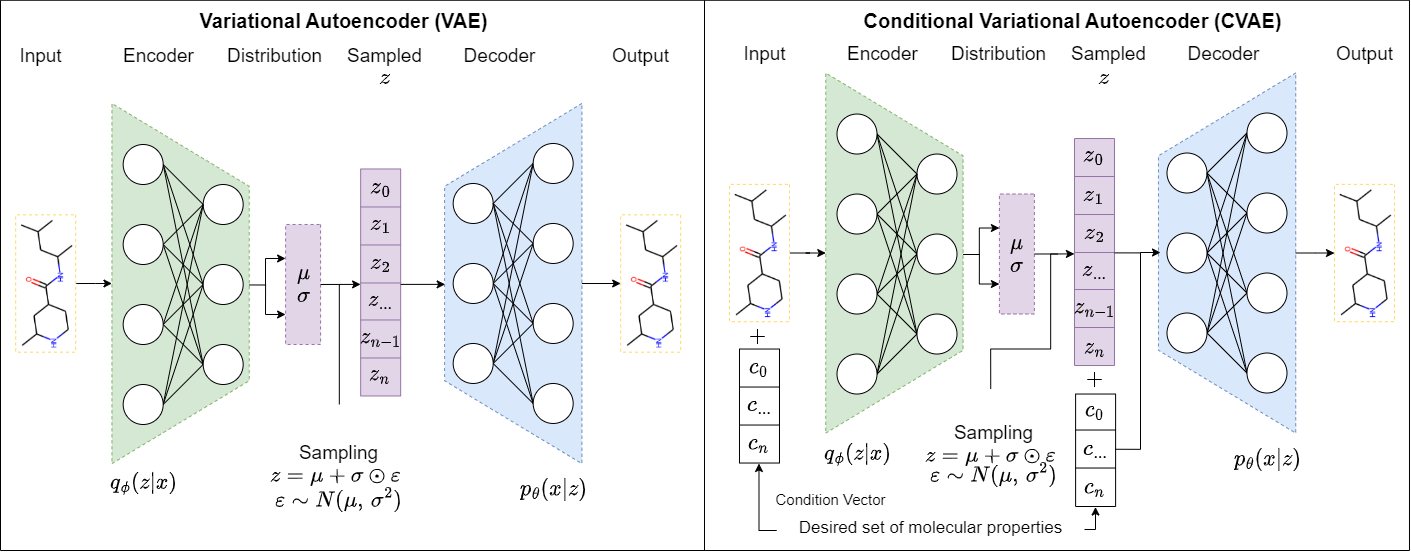
\includegraphics[width=1\textwidth]{fig1.png}
    \caption{Left: The VAE aims to reconstruct a new molecule similar to the input. Right: In a conditioned generation, the desired properties are introduced as explicit inputs to the model. The CVAE aims to reconstruct a new molecule with targeted and optimized molecular properties given the condition vector.}
    \label{fig:img1}
\end{figure*}


\subsection{Conditional VAE}
A conditional variational autoencoder (CVAE) is a generative model that is similar to a VAE but with the addition of conditioning information \cite{lim2018molecular}. The conditioning information directs the VAE to generate molecules with desired properties. The CVAE could be trained on a data set of molecules with known physical properties to generate novel compounds with similar properties by controlling the latent space dimensions that correspond to those properties. The CVAE could also be conditioned on additional information, such as desired chemical functionalities or substructures, to further control the generated compounds.
\begin{equation}
    \begin{split}
        \mathbb{E}_{q_\phi(z|x,c)}[log p_\theta(x|z),c] - D_{KL}[q_\phi(z|x,c)\parallel p(z|c)]. \label{eq}
    \end{split}
\end{equation}

The main difference between the objective function of a VAE in (3) and a CVAE in (5) is the condition vector, $c$. The condition vector corresponds to the targeted molecular properties that the model should learn when generating molecules. To that end, the decoder of the trained CVAE model would be able to generate molecules with the specified properties by using the condition vector with the latent vector\cite{lee2022mgcvae}.

\section{Property optimization}
The primary goal of \textit{de novo} drug discovery is to generate novel molecules whose specified molecular properties are optimized. The Ghose filter proposed in \cite{ghose1999knowledge} is a set of rules used to prioritize chemical compounds with potential pharmacological properties, such as drug-like behavior, lipophilicity, hydrogen bonding potential, and the presence of certain functional groups. \cite{wildman1999prediction} concurs with \cite{ghose1999knowledge} by providing a computational method for predicting the physicochemical parameters of chemical compounds using atomic contributions. These parameters, such as lipophilicity and hydrogen bonding potential, could be used to evaluate the potential of a compound to be a successful drug candidate based on its ability to interact with biological targets, its pharmacokinetic properties, and its potential for toxicity. This computational method is known as Crippen's method, which is widely used for the prediction of logP and MR \cite{wildman1999prediction}. RDKit provides the software implementation of their method for practical applications \cite{landrum2013rdkit}.

Crippen's logP (ClogP) is a measure that reflects the distribution of a molecule between an aqueous and an organic phase, with higher values indicating greater hydrophobicity. It is calculated based on the molecular structure of a compound and is used to predict its bioavailability and solubility. Crippen's molar refractivity (CMR) is a measure of the polarizability of a molecule, which is related to its electron density distribution. The CMR is used to predict physical properties such as boiling point and surface tension. Both ClogP and CMR are commonly used to evaluate potential drug candidates and design compounds with desired properties.

Recently, \cite{jin2018junction} introduced the penalized logP (plogP), which is a modified version of ClogP that takes into account functional groups that may affect the octanol-water partition coefficient value. The plogP aims to provide a more accurate prediction of solubility and bioavailability. While penalized logP may be considered more accurate in terms of measuring hydrophobicity or hydrophilicity, the choice between the two depends on the specific needs of the application and the availability of data. In some cases, Crippen logP may be sufficient, while in others, the use of penalized logP may be more appropriate.

Other optimization properties include the quantitative estimate of drug-likeness (QED) and synthetic accessibility score (SAS). QED is a quantitative measure that reflects the likelihood of a compound is a successful drug candidate based on its molecular structure. It is calculated using properties such as molecular weight, polar surface area, and lipophilicity \cite{craig1998molecular}. SAS is a measure of the ease with which a compound can be synthesized based on its molecular structure, taking into account factors such as the number of atoms, rotatable bonds, and rings in the molecule \cite{ertl2009estimation}. Both QED and SAS are frequently used in drug discovery to assess the potential of a compound as a drug candidate and to guide the selection of compounds for further development, often in conjunction with other molecular properties like biological activity and toxicity \cite{lee2022mgcvae}.

\section{Molecular fingerprints}
\subsection{Construction}
Morgan fingerprints are a type of molecular descriptor that captures information about the molecular structure and the connectivity of atoms in a molecule. They are generated by converting a molecule into a graph representation, where each atom is represented as a node and each bond is represented as an edge. The fingerprint is then generated by traversing the graph and counting the number of times a particular substructure is encountered.

In a Morgan fingerprint, the substructure is defined as a circular substructure of atoms and bonds, centered around a specific atom (the "root" atom). The circular substructure is generated by expanding the root atom to its neighboring atoms and bonds, and then expanding each of those atoms and bonds in the same manner, until a predefined size limit is reached. The size limit is typically set to a small number of bonds, such as 4 or 6, which results in a compact representation that captures the local molecular environment around each atom.

The count of each circular substructure is recorded in a binary vector, where each entry in the vector corresponds to a unique circular substructure. The binary value is set to 1 if the substructure is encountered in the molecule, and 0 otherwise. The final Morgan fingerprint is the concatenation of these binary vectors for each root atom in the molecule.

Morgan fingerprints are commonly used in cheminformatics and computational biology because they are computationally efficient, easy to generate, and provide a compact representation of molecular structure that is well-suited for comparison and search tasks.

\subsection{Tanimoto similarity}
Morgan fingerprints are used to detect molecular similarity by comparing the binary representations of the fingerprints of two molecules. The comparison can be performed using various similarity measures, such as Tanimoto similarity, Jaccard similarity, or Dice similarity.

In general, the Tanimoto similarity measure is the most commonly used similarity measure for Morgan fingerprints, as it provides a good balance between sensitivity and specificity. The Tanimoto similarity between two fingerprints is defined as the number of bits that are set to 1 in both fingerprints, divided by the total number of bits set to 1 in either fingerprint. A Tanimoto similarity value of 1 indicates that the two fingerprints are identical, while a value of 0 indicates that the fingerprints have no bits in common.

The Tanimoto similarity can be calculated efficiently using bitwise operations, making it well-suited for large-scale molecular comparison tasks. In addition, the binary representation of Morgan fingerprints makes it possible to use fast indexing and search algorithms, such as MinHash and LSH, to speed up molecular similarity search.

By comparing the Morgan fingerprints of two molecules, one can determine the degree of molecular similarity between them, and use this information to classify and predict molecular properties, such as bioactivity, toxicity, and solubility.

\subsection{Validity, novelty, and uniqueness (V.N.U)}
Morgan fingerprints can be used to assess the validity, novelty, and uniqueness of generated molecules in computational chemistry and molecular design.

\subsubsection{Validity}
Validity refers to the chemical feasibility of a molecule, and whether it violates any basic chemical rules or constraints, such as bond valences or molecular formula. To assess the validity of a generated molecule, one can compare its Morgan fingerprint to a reference set of fingerprints from known, valid molecules. If the generated molecule has a similar fingerprint to a known valid molecule, it is likely to be chemically feasible.

\subsubsection{Novelty}
Novelty refers to the degree of uniqueness of a molecule compared to a reference set of known molecules. To assess the novelty of a generated molecule, one can compare its Morgan fingerprint to the fingerprints of the known molecules and calculate the Tanimoto similarity. If the generated molecule has a low Tanimoto similarity to any known molecule, it is considered to be novel.

\subsubsection{Uniqueness}
Uniqueness refers to the degree of uniqueness of a molecule compared to a set of already generated molecules. To assess the uniqueness of a generated molecule, one can compare its Morgan fingerprint to the fingerprints of the previously generated molecules and calculate the Tanimoto similarity. If the generated molecule has a low Tanimoto similarity to any of the previously generated molecules, it is considered to be unique.

By using Morgan fingerprints to assess the validity, novelty, and uniqueness of generated molecules, one can ensure that the generated molecules are chemically feasible, and have the desired level of novelty and uniqueness for a specific application or project.

\subsubsection{Morgan fingerprint limitations}
There are several limitations to using Morgan fingerprints for molecular similarity and molecular design:

Size limitations: Morgan fingerprints have a limited size, which means that they may not capture all the details of a molecular structure, particularly for large and complex molecules.

Lack of geometric information: Morgan fingerprints do not encode information about the three-dimensional shape of a molecule, which is important for molecular interactions and properties.

Overgeneralization: The circular substructures used in Morgan fingerprints can result in overgeneralization, where similar molecules with different chemical properties are assigned similar fingerprints.

Bit-level granularity: The binary representation of Morgan fingerprints has a limited granularity, as each bit can only be 0 or 1. This means that the fingerprints do not encode information about the relative strength of different molecular features.

Computational cost: Generating Morgan fingerprints can be computationally expensive, particularly for large and complex molecules.

Despite these limitations, Morgan fingerprints are still widely used in molecular similarity and molecular design due to their simplicity, efficiency, and robustness. To overcome some of these limitations, alternative molecular descriptors, such as molecular graphs and graph convolutional neural networks, have been developed and are becoming increasingly popular.

\section{Limitations}
Recent works on CVAEs have shown great success in generating molecules with targeted properties through the conditioning vector. However, prior research has found that CVAEs may struggle to effectively separate the latent molecular representations \cite{richards2022conditional}. To overcome this limitation, we introduce disentanglement to the CVAE in (5) with the $\beta$ hyperparameter presented in (4). This paper introduces the molecular graph $\beta$-CVAE model for \textit{de novo} drug discovery. 

\section{Contribution}
 The simultaneous optimization of molecules with multiple properties remains a significant challenge. By introducing a conditional vector to the latent space of the $\beta$-VAE, we aim to generate novel molecules by the following contribution: 
\begin{enumerate}
\item we proposed a molecular graph $\beta$-CVAE model to generate novel molecules;
  \item we increased the maximum molecule length of 16 in \cite{lee2022mgcvae} to 18;
  \item we applied a hyper-hyperparameter gradient descent training of our models proposed in \cite{DBLP:journals/corr/abs-1909-13371}.
\end{enumerate}
